% ==============================================================================
% Chapter 3: Market Risk Quantification via Value at Risk (VaR) & Backtesting
% ==============================================================================

\chapter{Market Risk Measurement via Value at Risk (VaR)}
\label{ch:var_modeling}

\section{Theoretical Foundations and Mathematical Formulation of VaR}
\label{sec:var_foundations}

Value at Risk ($\VaR$) is the standard benchmark metric adopted by international regulatory frameworks (Basel II/III) and institutional investment managers to quantify downside market risk. Formally, $\VaR$ measures the maximum potential capital loss that an investment portfolio is expected to suffer over a specified holding period $T_h$, at a designated statistical confidence level $1 - \alpha$, under normal market conditions.

\begin{definition}{Value at Risk ($\VaR$)}{var_definition}
Let $\Delta V = V(t + T_h) - V(t)$ represent the profit or loss ($\text{P\&L}$) of a financial portfolio over holding horizon $T_h$, where $V(t)$ is the initial portfolio value. For a given significance level $\alpha \in (0, 1)$, the Value at Risk $\VaR_{\alpha, T_h}$ is defined as the negative of the $\alpha$-quantile of the $\text{P\&L}$ distribution:
\begin{equation}
\VaR_{\alpha, T_h} = -\inf \left\{ \ell \in \mathbb{R} : \Prob\left(\Delta V \le \ell\right) > \alpha \right\}
\label{eq:var_general}
\end{equation}
Equivalently, in terms of percentage portfolio returns $\mathcal{R} = \Delta V / V_0$:
\begin{equation}
\Prob\left(\mathcal{R} \le -\VaR_{\%}\right) = \alpha \quad \iff \quad \Prob\left(\Delta V \le -V_0 \cdot \VaR_{\%}\right) = \alpha
\end{equation}
\end{definition}

While $\VaR$ provides an intuitive, single-number summary of market exposure, it possesses theoretical limitations: specifically, it is not a \textit{coherent risk measure} in the sense of Artzner et al. (1999) because it fails the axiom of \textbf{subadditivity} ($\VaR(X + Y) \le \VaR(X) + \VaR(Y)$ does not hold in non-elliptical or highly skewed distributions). To remediate this deficit, risk managers complement $\VaR$ with \textbf{Expected Shortfall ($\ES$)}, also termed Conditional Value at Risk ($\CVaR$):
\begin{equation}
\CVaR_{\alpha, T_h} = -\E\left[ \Delta V \;\middle|\; \Delta V \le -\VaR_{\alpha, T_h} \right]
\label{eq:cvar_general}
\end{equation}
$\CVaR$ is strictly subadditive and quantifies the expected magnitude of loss in the event that an extreme tail breach occurs.

\section{Parametric (Delta-Normal) VaR Model}
\label{sec:parametric_var}

The Parametric (or Variance-Covariance) approach assumes that daily continuously compounded returns follow a stationary Gaussian distribution: $R_t \sim \mathcal{N}(\mu, \sigma^2)$. Under this assumption, the 1-day percentage $\VaR$ at confidence level $1 - \alpha$ is given by:
\begin{equation}
\VaR_{\text{param}, 1-\alpha}^{1\text{d}} = Z_{\alpha} \cdot \sigma_{\text{daily}} - \mu_{\text{daily}}
\label{eq:parametric_1d}
\end{equation}
where $Z_{\alpha} = \Phi^{-1}(1 - \alpha)$ represents the standard normal critical value ($Z_{0.05} = 1.644853$ for $95\%$ confidence, and $Z_{0.01} = 2.326348$ for $99\%$ confidence). In Rupee terms, for an initial portfolio position of $V_0$:
\begin{equation}
\VaR_{\text{param}, 1-\alpha}^{1\text{d}} (\text{\rupee}) = V_0 \cdot \left( Z_{\alpha} \cdot \sigma_{\text{daily}} - \mu_{\text{daily}} \right)
\label{eq:parametric_1d_inr}
\end{equation}

\subsection{Multi-Period Scaling: The Square-Root of Time Rule}

To evaluate risk over longer institutional horizons (such as the standard 10-day horizon mandated by the Basel Committee for market risk capital charges), risk managers scale 1-day estimates using the \textbf{Square-Root of Time rule}:
\begin{equation}
\VaR_{\alpha, T_h} = \VaR_{\alpha, 1\text{d}} \times \sqrt{T_h}
\label{eq:sqrt_time}
\end{equation}

\begin{theorem}{Square-Root of Time Scaling Validity}{sqrt_time_theorem}
Let cumulative multi-period return over $T_h$ days be $R_{t, t+T_h} = \sum_{j=1}^{T_h} R_{t+j}$. If the daily return series $\{R_t\}$ is independent and identically distributed ($\text{i.i.d.}$) with mean $\mu \approx 0$ and constant variance $\sigma^2$, then:
\begin{equation}
\Var\left(R_{t, t+T_h}\right) = \sum_{j=1}^{T_h} \Var(R_{t+j}) = T_h \cdot \sigma^2 \implies \sigma_{T_h} = \sigma_{\text{daily}} \sqrt{T_h}
\end{equation}
Consequently, quantile scaling preserves linearity: $\VaR_{T_h} = \VaR_{1\text{d}} \sqrt{T_h}$.
\end{theorem}

\begin{remarkbox}[Validity Caveat of the $\sqrt{T_h}$ Rule]
The $\sqrt{T_h}$ scaling rule strictly holds only when returns are uncorrelated ($\Cov(R_t, R_{t-k}) = 0$). In the presence of volatility clustering (GARCH effects) or mean reversion, scaling by $\sqrt{T_h}$ can distort multi-day risk forecasts. Nevertheless, it remains the standard regulatory benchmark across global clearing corporations and exchanges.
\end{remarkbox}

\section{Non-Parametric Historical Simulation VaR}
\label{sec:historical_var}

Unlike the parametric approach, \textbf{Historical Simulation $\VaR$} makes zero assumptions regarding the underlying probability density function. Instead, it lets the empirical price history speak for itself by sorting the observed historical returns $\{R_t\}_{t=1}^N$ in ascending order:
\begin{equation}
R_{(1)} \le R_{(2)} \le \dots \le R_{(N)}
\end{equation}
The empirical 1-day $\VaR$ at confidence level $1 - \alpha$ corresponds directly to the empirical $\alpha$-percentile of the sample:
\begin{equation}
\VaR_{\text{hist}, 1-\alpha}^{1\text{d}} = - Q_{\alpha}\left(\{R_t\}_{t=1}^N\right) = - R_{(\lceil N \alpha \rceil)}
\label{eq:historical_var}
\end{equation}
Similarly, empirical Expected Shortfall is computed as the arithmetic mean of all historical observations that fall below the $\VaR$ cutoff:
\begin{equation}
\CVaR_{\text{hist}, 1-\alpha}^{1\text{d}} = - \frac{1}{\lfloor N \alpha \rfloor} \sum_{t=1}^{\lfloor N \alpha \rfloor} R_{(t)}
\label{eq:historical_cvar}
\end{equation}
Multi-period historical estimates are scaled via $\sqrt{T_h} = \sqrt{10} \approx 3.162278$.

\section{Empirical Exposure Results on 1 Lot of ITC Shares}
\label{sec:empirical_var_results}

We now calibrate both models to an equity portfolio holding exactly \textbf{1 standard NSE F\&O market lot} of ITC Limited:
\begin{itemize}
    \item \textbf{Lot Size ($L$):} $1,725$ shares (standard NSE derivative lot for November/December 2026 contracts).
    \item \textbf{Spot Price ($S_0$):} \rupee 285.00 per share.
    \item \textbf{Total Market Capital Commitment ($V_0$):} $1,725 \times \text{\rupee}285.00 = \text{\textbf{\rupee 4,91,625.00}}$ ($\approx \text{\rupee}4.92\text{ lakh}$).
    \item \textbf{Sample Diagnostics:} $N = 246$, $\hat{\mu} = -0.001114$, $\hat{\sigma} = 0.014742$ ($23.40\%$ annualized).
\end{itemize}

Table~\ref{tab:var_results} provides the comprehensive empirical risk quantification across all confidence levels and holding periods.

\begin{table}[htbp]
\centering
\small
\caption{Empirical Value at Risk ($\VaR$) and Expected Shortfall ($\CVaR$) for 1 Lot of ITC ($V_0 = \text{\rupee}4,91,625$)}
\label{tab:var_results}
\begin{tabularx}{\linewidth}{lXrrrr}
\toprule
\textbf{Risk Metric} & \textbf{Model Methodology} & \textbf{1-Day (\%)} & \textbf{1-Day (INR)} & \textbf{10-Day (\%)} & \textbf{10-Day (INR)} \\
\midrule
$\VaR_{95\%}$ & Parametric (Delta-Normal) & $2.54\%$ & \rupee 12,468.81 & $8.02\%$ & \rupee 39,429.84 \\
$\VaR_{95\%}$ & Historical Simulation & $2.09\%$ & \rupee 10,296.51 & $6.62\%$ & \rupee 32,560.44 \\
\midrule
$\VaR_{99\%}$ & Parametric (Delta-Normal) & $3.54\%$ & \rupee 17,407.90 & $11.20\%$ & \rupee 55,048.61 \\
$\VaR_{99\%}$ & Historical Simulation & $3.96\%$ & \rupee 19,443.90 & $12.51\%$ & \rupee 61,487.02 \\
\midrule
$\CVaR_{95\%}$ & Historical Expected Shortfall & $3.51\%$ & \rupee 17,264.03 & $11.10\%$ & \rupee 54,593.64 \\
$\CVaR_{99\%}$ & Historical Expected Shortfall & $6.12\%$ & \rupee 30,083.04 & $19.35\%$ & \rupee 95,130.94 \\
\bottomrule
\end{tabularx}
\end{table}

\begin{empiricalbox}{The Fat-Tail Wedge: Parametric vs. Historical Tail Discrepancy}{fat_tail_wedge}
At the $95\%$ confidence level, Parametric $\VaR$ (\rupee 12,468.81) is actually \textit{higher} than Historical $\VaR$ (\rupee 10,296.51) due to the central leptokurtic peakedness of the empirical return distribution. 

However, at the extreme $99\%$ tail, the relationship dramatically inverts:
\begin{equation}
\VaR_{\text{hist}, 99\%}^{10\text{d}} = \text{\textbf{\rupee 61,487.02}} \quad \text{vs.} \quad \VaR_{\text{param}, 99\%}^{10\text{d}} = \text{\textbf{\rupee 55,048.61}}
\end{equation}
Historical Simulation produces an unhedged 10-day downside risk estimate that is \textbf{\rupee 6,438.41 higher (+11.70\%)} than the parametric Gaussian estimate. Furthermore, the 10-day $99\%$ Expected Shortfall reaches \textbf{\rupee 95,130.94} ($19.35\%$ of total capital), exposing the catastrophic drawdown risk lurking in the empirical tail that Gaussian models completely overlook.
\end{empiricalbox}

\section{Model Validation via Kupiec POF Backtesting}
\label{sec:kupiec_backtesting}

A risk model cannot be deployed in institutional practice without empirical backtesting. The regulatory standard for backtesting is the \textbf{Kupiec Proportion of Failures ($\POF$) test} (Kupiec, 1995), which assesses whether the observed failure rate of a model is statistically consistent with its nominal coverage probability.

\begin{definition}{Kupiec Likelihood Ratio ($\LR_{\POF}$) Statistic}{kupiec_definition}
Let $N$ be the total number of historical trading days, and let $x$ denote the number of days on which actual daily loss exceeded the predicted 1-day $\VaR$ threshold (termed an \textit{exception} or \textit{violation}):
\begin{equation}
x = \sum_{t=1}^{N} \mathbb{I}_{\{R_t < -\VaR_{\%}\}}
\end{equation}
Under the null hypothesis $H_0: p = p_0$ (where $p_0 = 1 - \text{Confidence Level} = 0.05$ or $0.01$), the sample failure rate is $\hat{p} = x / N$. The Likelihood Ratio test statistic is formulated as:
\begin{equation}
\LR_{\POF} = -2 \ln \left[ \frac{(1 - p_0)^{N - x} p_0^x}{(1 - \hat{p})^{N - x} \hat{p}^x} \right] = 2 \left[ x \ln\left(\frac{\hat{p}}{p_0}\right) + (N - x) \ln\left(\frac{1 - \hat{p}}{1 - p_0}\right) \right]
\label{eq:kupiec_lr}
\end{equation}
Asymptotically, $\LR_{\POF} \sim \chi^2(1)$. At the standard $5\%$ significance level ($\alpha_{\text{stat}} = 0.05$), the critical value is $\chi^2_{0.05, 1} = 3.8415$. If $\LR_{\POF} > 3.8415$, the null hypothesis is rejected, indicating that the $\VaR$ model either systematically underestimates risk (too many breaches) or is excessively conservative (too few breaches).
\end{definition}

\begin{table}[htbp]
\centering
\small
\caption{Kupiec POF Backtest Results for 1-Day VaR Models ($N = 246$ Days)}
\label{tab:kupiec_results}
\begin{tabularx}{\linewidth}{lXrrrrr}
\toprule
\textbf{Model Evaluated} & \textbf{Nominal $p_0$} & \textbf{Expected $x$} & \textbf{Observed $x$} & \textbf{Empirical $\hat{p}$} & \textbf{$\LR_{\POF}$ Stat} & \textbf{$p$-value} \\
\midrule
$95\%$ Parametric $\VaR$ & $0.050$ & $12.3$ & $9$ & $0.0366$ & $1.0236$ & $0.3117$ \\
$99\%$ Parametric $\VaR$ & $0.010$ & $2.5$ & $4$ & $0.0163$ & $0.8188$ & $0.3655$ \\
$95\%$ Historical $\VaR$ & $0.050$ & $12.3$ & $13$ & $0.0528$ & $0.0412$ & $0.8391$ \\
$99\%$ Historical $\VaR$ & $0.010$ & $2.5$ & $3$ & $0.0122$ & $0.1119$ & $0.7380$ \\
\bottomrule
\end{tabularx}
\end{table}

\begin{figure}[htbp]
\centering
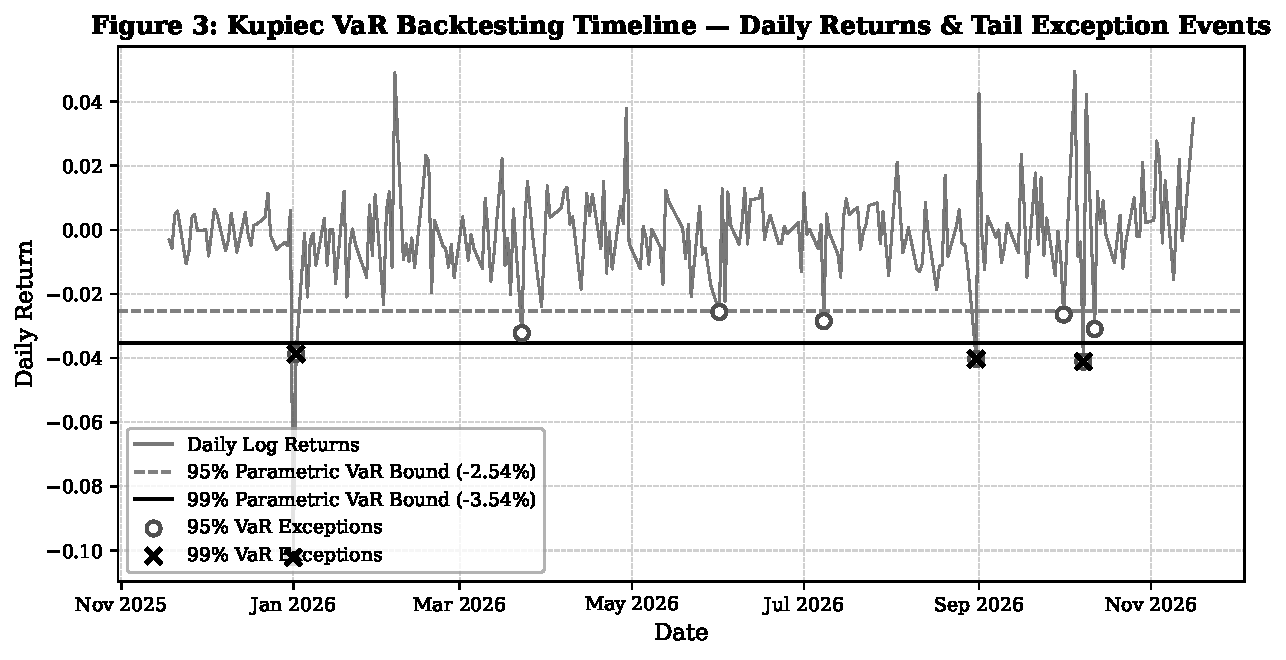
\includegraphics[width=0.96\linewidth]{figures/fig3_kupiec_backtesting.pdf}
\caption{Kupiec VaR Backtesting Timeline: Daily Return Series and Tail Violations}
\label{fig:kupiec_timeline}
\vspace{2pt}
\begin{minipage}{0.96\linewidth}
\footnotesize\textbf{Note:} Daily log returns of ITC plotted against the horizontal 1-day $95\%$ (dashed) and $99\%$ (solid) Parametric $\VaR$ boundaries. Circular markers indicate $95\%$ exception breaches ($x = 9$); cross markers designate extreme $99\%$ tail violations ($x = 4$).
\end{minipage}
\end{figure}

As documented in Table~\ref{tab:kupiec_results} and illustrated in Figure~\ref{fig:kupiec_timeline}, all four models successfully pass the Kupiec test at the $5\%$ significance level ($\LR_{\POF} < 3.8415$, $p$-values ranging from $0.31$ to $0.84$). 

Under the Basel Committee on Banking Supervision (BCBS) regulatory \textit{Traffic Light System} for 250-day backtesting at $99\%$ confidence:
\begin{itemize}
    \item \textbf{Green Zone ($0\text{--}4$ exceptions):} The model is deemed accurate and acceptable without regulatory capital penalty multipliers.
    \item \textbf{Yellow Zone ($5\text{--}9$ exceptions):} The model raises monitoring concerns; supervisory scaling multipliers increase from $3.0$ to $3.85$.
    \item \textbf{Red Zone ($\ge 10$ exceptions):} The model is categorically rejected.
\end{itemize}
With $x = 4$ exceptions under the Parametric model and $x = 3$ exceptions under Historical Simulation, both models reside safely within the \textbf{Green Zone}. However, because the historical simulation model accurately captures the empirical \rupee 61,487.02 10-day tail risk, we designate this figure as the unhedged benchmark loss to be insulated via derivative options in Chapter~\ref{ch:hedging}.
